\chapter{Avaliação}

  \section{Resultado das Avaliações}
  
     \section{Avaliação dos Protótipos de Papel}
     
     Para se realizar a avaliação do protótipo de papel, foi solicitado a 5 usuários com um perfil comum e compatível com a proposta do aplicativo 
  (frequentadores de eventos), que realizassem duas atividades:
  
  \begin{itemize}
       \item Criasse uma notificação com data e hora definidos.

       \item Gerenciasse suas notificações agendadas.
       
  \end{itemize}
     
        \section{Itens do questionário aplicado}
        
        Abaixo se encontram as perguntas, provenientes do questionário ASQ, após a realização das atividades solicitadas no protótipo de papel:
     
     1. No geral, estou satisfeito com a facilidade de completar das atividades neste cenário.
     2. No geral, estou satisfeito com a quantidade de tempo que levei para completar as atividades neste cenário.
     3. No geral, estou satisfeito com a informação de suporte (ajuda on-line, mensagens, documentação) fornecida enquanto completava as atividades.
     
     É importante salientar que as questões tinham como opção de resposta de 1 a 7 e a opção “Não se aplica”, sendo que 1 significa que o usuário concorda 
     fortemente com o que está sendo perguntado e 7 que o usuário discorda fortemente.
  
        \section{Resultados da primeira avaliação}
        
        Na figura abaixo, se encontram as notas atribuídas pelos cinco usuários, sendo que foram realizadas as atividades dos cenários A e B já citadas e 
        feitas as três questões também descritas.
        
        
        
        
        \begin{figure}[!htb]
        \centering
        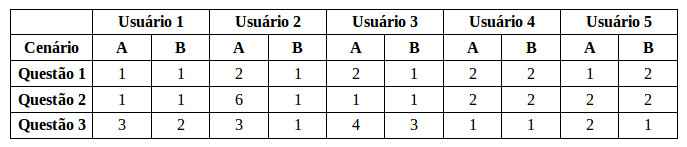
\includegraphics[scale=0.6]{figuras/nota1avaliacao.jpg}
        \caption{Notas atribuídas por usuários na primeira avaliação do protótipo de papel}
        \end{figure}
        
        
        
             
        
	Além da atribuição da nota, tambem houve outro feedback por parte dos usuários, sendo que este foi feito por descreverem o que sentiram falta na aplicação, 
	dados exibidos abaixo:
	
	\textbf{Usuário 1}
	
	Sentiu falta de:
	
	 \begin{itemize}
       \item Um campo para escolher a cidade do evento na tela de escolher para quando deseja a notificação.

       \item Mensagem de confirmação de exclusão de uma notificação.
       
        \end{itemize}
	
	
	\textbf{Usuário 2}
	
	Sentiu falta de:
	
	\begin{itemize}
       \item Mensagem de notificação da perda dos dados caso queira voltar para uma tela anterior.

       \item A possibilidade de escolher um intervalo de horário para a notificações, ao invés de um horário fixo.
       
       \item Ao invés de colocar a mensagem de confirmação do salvamento de uma notificação em uma tela separada, colocar como uma mensagem sobrepondo a mesma tela.

       \item As notificações agendadas poderiam aparecer logo na página inicial.
       
        \end{itemize}
	
	\textbf{Usuário 3}
	
	Sentiu falta de:
	
	\begin{itemize}
       \item Uma melhor visualização do campo que exibe as notificações adicionadas.

       \item Lista de notificações agendadas mais centralizada.
       
       \item Símbolo de “Retirar tema” mais intuitivo.

       \item Caixinha de “Mais temas” na tela de edição.
       
        \end{itemize}
	
	\textbf{Usuário 4}
	
	Sentiu falta de:
	
	\begin{itemize}
       \item Especificação que a notificação de horário é referente a notificação.

       \item Melhorar símbolo de “menos” do “Editar notificação”.
       
        \end{itemize}
	
	\textbf{Usuário 5}
	
	Sentiu falta de:
	
	\begin{itemize}
       \item Espaço para comentários sobre uma notificação. Ex: Comprar ingresso para a tia Tânia.
       
        \end{itemize}
  
        \section{Análise dos resultados obtidos na avaliação}
        
        De modo geral, o feedback recebido foi positivo e por ter sido adotado o questionário ASQ foi obtido um retorno capaz de fornecer 
        uma medição mais precisa a medida que o projeto for evoluindo. Também por meio do uso do questionamento sobre o que foi sentido falta, 
        foi obtido um feedback rápido sobre a opinião do usuário em relação as melhorias necessárias.
  